\section{Architettura}
%descrizione generale del progetto
Per la progettazione del componente si è scelto di utilizzare un architettura modulare divisa in un'unità di elaborazione (Data path) e un'unità di controllo (FSM).

Da un'ottica di alto livello, l'implementazione esegue i seguenti passi:
\begin{enumerate}
\item carico nel primo registro il valore della prima cella di memoria
\item carica nel secondo registro il valore della seconda cella di memoria
\item calcola la dimensione dell'immagine utilizzando un blocco che conta i pixel
\item legge 1 ad 1 tutti i pixel dell'immagine e ne calcola massimo e minimo
\item calcola il delta tra massimo e minimo, il log e lo shift\_level come da specifica
\item esegue lo shift e scrive a partire dal primo indirizzo di memoria libero i valori dei nuovi pixel, calcolati come da specifica calcolando MIN( 255 , TEMP\_PIXEL)
\end{enumerate}

Per la realizzazione del modulo sono stati utilizzati registri di tipo parallelo-parallelo che aggiornano il proprio contenuto sul fronte di salita del clock. 
Tutti i registri sono stati definiti in VHDL con approccio behaviuoral tramite Process e hanno tutti sensitivity list (i\_rst, i\_clk) e, in caso di reset (asincrono), vengono resettati al valore '0'.

%%%%%%%%%%%%
\subsection{Datapath}
In questa sezione è descritto il DataPath dividendone la trattazione in moduli logici dedicati ad eseguire specifici tasks.

\begin{enumerate}
\item calcolo dimensione immagine
\item gestione indirizzi
\item esecuzione algoritmo
\end{enumerate}

\subsubsection{Calcolo dimensione immagine} 
Questo modulo è composto da 2 registri, \texttt{registro\_1} e \texttt{registro\_2} (realizzati come specificato precedentemente) che memorizzano rispettivamente il primo e secondo Byte di memoria.
A seguire sono presenti un sommatore, un sottrattore, un comparatore e un registro (\texttt{regTS})  che combinati consentono di calcolare per somme successive il numero di pixel totali dell'immagine.

%, per mezzo di un algoritmo a somme successive,

 A cascata è presente un ulteriore sommatore che, alla fine del conteggio, incrementa di 1 il valore presente in \texttt{regTS}\footnote{\texttt{la sensitivity list}, a differenza degli altri registri, comprende anche il segnale \texttt{i\_start} per permettere la reinizializzazione di questo specifico registro ogni volta che viene sottoposta al modulo una nuova immagine}. Questo valore è infine salvato nel registro \texttt{reg sum\_1} che viene portato in ingresso ad un comparatore e ad un multiplexer usati, come descritto di seguito, nel modulo di gestione indirizzi.

%%%%%%%%%
In questo modulo vengono generati 3 segnali d'uscita: \texttt{finish}, \texttt{o\_end} e \texttt{CZ}. I primi 2 hanno lo scopo di gestire 2 dei casi limite (verranno approfinditi di seguito) mentre il terzo é utilizzato per notificare la conclusione del processo che permette di contare i pixel presenti nell'immagine.



\subsubsection{Gestione indirizzi}
La gestione degli indirizzi è realizzata mediante 2 cicli di conteggio e un multiplexer.
Un ciclo é adibito al conteggio degli indirizzi di lettura (quello che in Figura \ref{Datapath} comprende il \texttt{registro count}), l'altro agli indirizzi di scrittura (Figura \ref{Datapath} ciclo che comprende \texttt{reg sum\_2)}. Tramite il multiplexer si può decidere da quale dei 2 cicli attingere l'indirizzo da mandare alla memoria per mezzo del segnale \texttt{addr\_sel}.

\newpage

Il ciclo di conteggio degli indirizzi è composto di:
\begin{itemize}
\item un multiplexer per l'inizializzazione dei registri
\item un sommatore a 16 bit che incrementa di 1 l'indirizzo ogni volta che \texttt{rco\_load}='1' e \texttt{rsu\_load}='1' rispettivamente
\item un registro per memorizzare l'indirizzo
\end{itemize}

Il segnale \texttt{o\_end}, che consente di terminare la fase di lettura e passare a quella di elaborazione, viene alzato nel momento in cui l'indirizzo corrente diventa uguale a quello memorizzato nel registro \texttt{reg sum\_1}.

Tutti i multiplexer sono stati realizzati in VHDL utilizzando il costrutto with-select.


\subsubsection{Esecuzione algoritmo}
Questo terzo modulo é quello adibito all'esecuzione dell'algoritmo vero e proprio.

Massimo e minimo sono implementati mediante 1 comparatore, 2 multiplexer e 1 registro.
Il comparatore confronta ad ogni ciclo il valore in ingresso su i\_data con quello memorizzato nel registro max/min e se i\_data è rispettivamente maggiore/minore viene memorizzato nel registro corrispondente, altrimenti viene mantenuto il valore precedente.
Alla fine della lettura dell'intera immagine, nei due registri (\texttt{registro max} e \texttt{registro min}) avrò memorizzato massimo e minimo, pronti per essere utilizzati per i calcoli successivi.\\

Vengono poi calcolati:

\begin{enumerate}
    \item \texttt{DELTA\_VALUE = MAX\_PIXEL\_VALUE – MIN\_PIXEL\_VALUE};
    \item \texttt{Y = FLOOR(LOG2(DELTA\_VALUE +1))};
    \item \texttt{SHIFT\_LEVEL = (8 – Y)};
\end{enumerate}


Questa fase si conclude calcolando per ogni pixel:
\begin{enumerate}
    \item[4.]  \texttt{TEMP\_PIXEL = (CURRENT\_PIXEL\_VALUE - MIN\_PIXEL\_VALUE) << SHIFT\_LEVEL};
\end{enumerate}

e assegnando il nuovo valore ad esso nel seguente modo
\begin{enumerate}
    \item[5.]   \texttt{NEW\_PIXEL\_VALUE = MIN( 255 , TEMP\_PIXEL)};
\end{enumerate}





per poi infine scriverlo in memoria.\\

Considerando la limitatezza del loro codominio, le funzioni di floor\_log e shift ("<<") sono state realizzate mediante dei process che mappano in maniera diretta il valore d'ingresso sul corrispondente valore in uscita.

%immagine Datapath
\begin{figure}[ht]
    \centering
    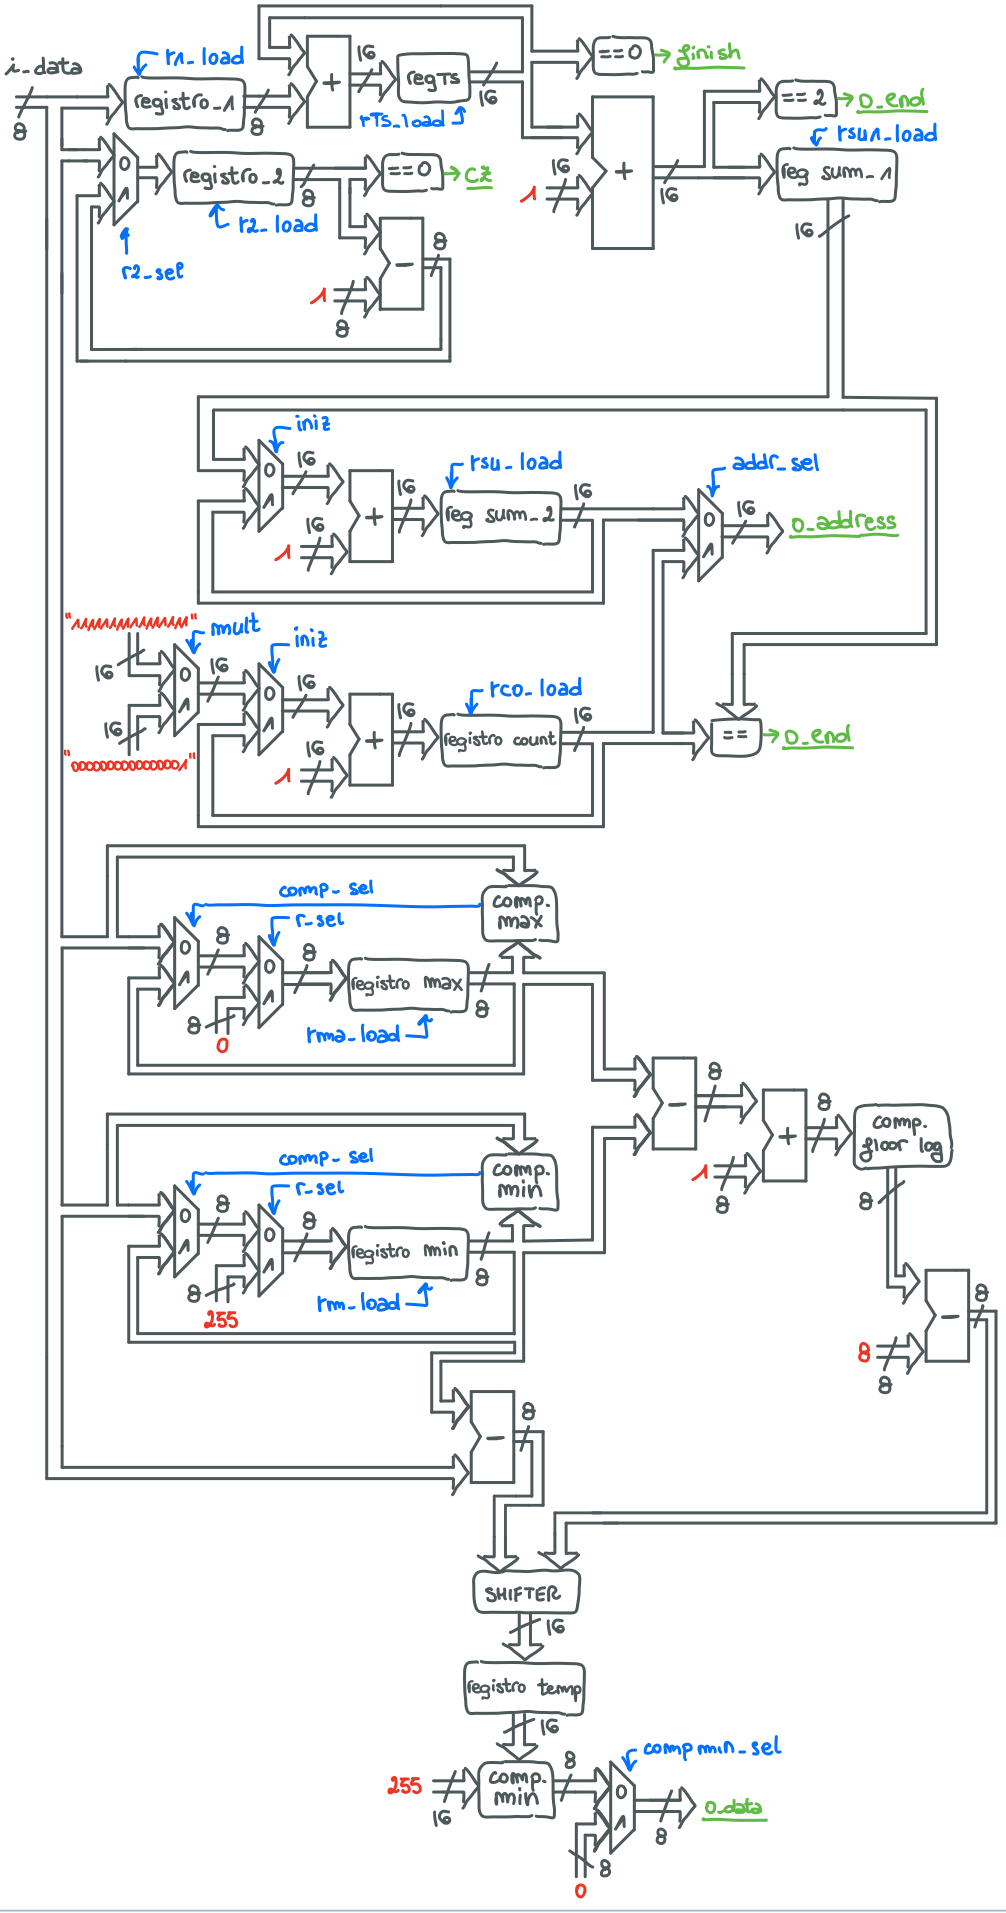
\includegraphics[scale = 0.34]{Figure/Datapath} 
    \caption{Datapath}
    \label{Datapath}
\end{figure}

\clearpage





\subsection{Macchina a Stati}

Si è scelto di utilizzare una sequenza di esecuzione separata per la gestione dei casi limite; questo per consentire il controllo di alcuni segnali parallelamente alla normale esecuzione, aumentandone la velocità nei suddetti casi. 

\begin{figure}[ht]
    \centering
    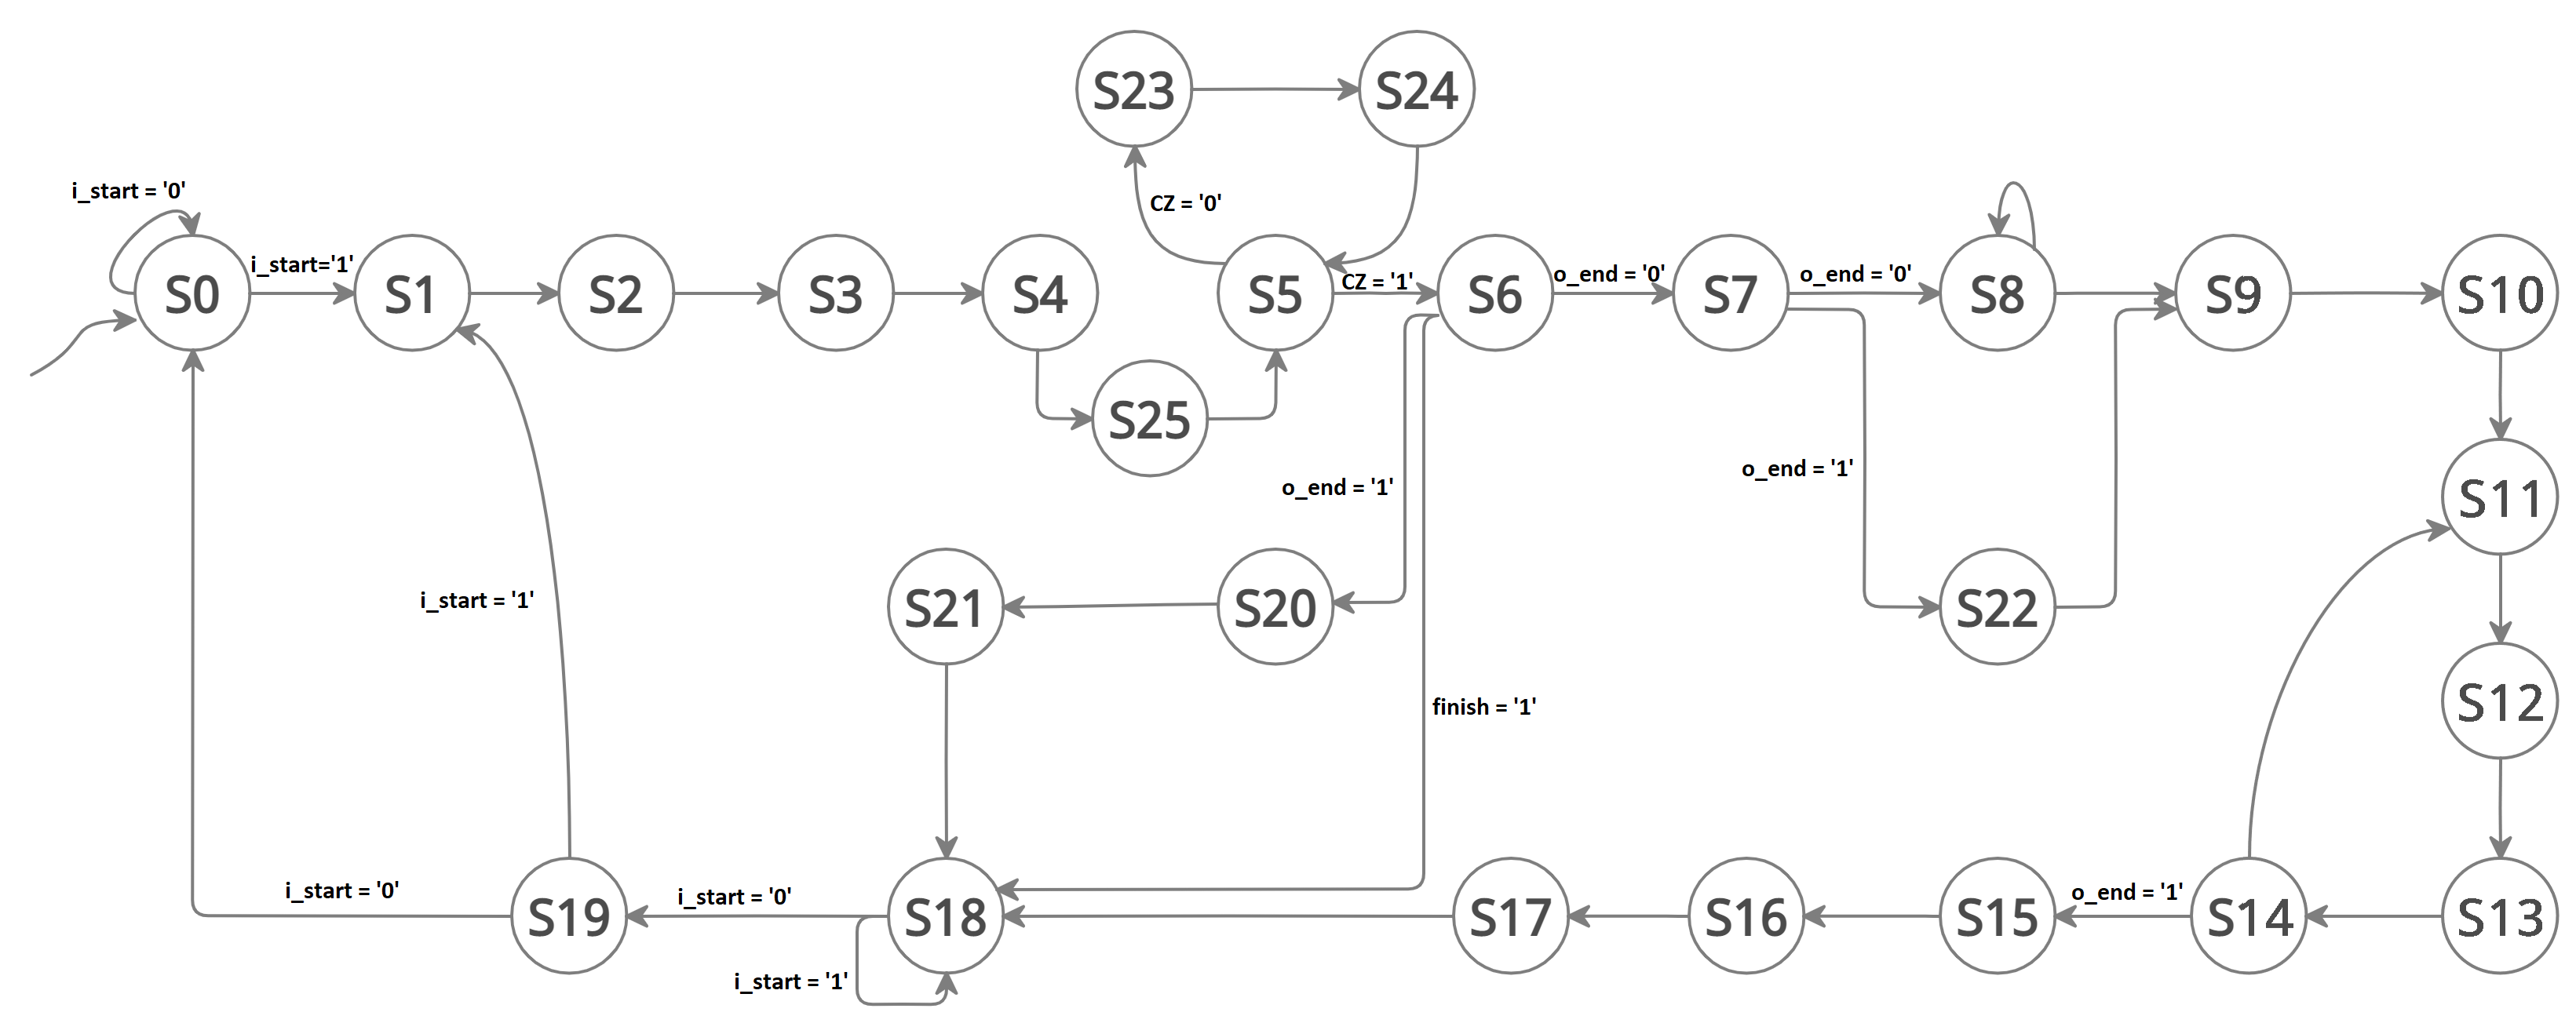
\includegraphics[scale = 0.182]{Figure/macchina a stati}
    \caption{Macchina a stati}
    \label{ms}
\end{figure}

\textit{\underline{oss}: E' stato assegnato il valore 0 come default a tutti i segnali della macchina a stati.}\\

Di seguito é riportata una breve descrizione per ogni stato della FSM:
\begin{itemize}
    \item[\textbf{S0}:]Stato di reset. Permette di attendere che l'equalizzazione abbia inizio. Si rimane in questo stato finché \texttt{i\_start} non viene alzato per passare quindi \textbf{S1};
    \item[\textbf{S1}:]Carica il registro \texttt{reg\_count} con il primo indirizzo di memoria ponendo \texttt{rco\_load}='1'; 
    \item[\textbf{S2}:]Inizializza il registro \texttt{reg\_max} a '0' e il registro \texttt{reg\_min} a '255'. Inoltre incrementa di 1 il valore memorizzato in \texttt{reg\_count} alzando il segnale \texttt{rco\_load} (quest'ultimo passaggio verrá ripetuto per incrementare gli indirizzi quando necessario);
    \item[\textbf{S3-S4}:] Consentono di immagazzinare il contenuto della prima e della seconda cella di memoria  rispettivamente nei registri \texttt{reg\_1} e \texttt{reg\_2}. Per farlo poniamo ad '1' i seguenti segnali: \texttt{r1\_load}, \texttt{r2\_load}, \texttt{o\_en}, \texttt{iniz}, \texttt{rco\_load};  

    \item[\textbf{S25}:]Introdotto per il corretto funzionamento del ciclo che permette di calcolare la dimensione dell'immagine. Consente al registro \texttt{reg2} di propagare il valore memorizzato nello stato precedente in uscita; 
    
    \item[\textbf{S5-S23-S24}:] Il ciclo composto da questi stati permette di calcolare il numero di pixel presenti nell'immagine. Viene portato avanti fino a che il contenuto del registro \texttt{reg\_2} é diverso da zero, appena questa condizione viene violata il segnale \texttt{CZ} viene alzato e da \textbf{S5} si passa ad \textbf{S6}. 
    Nel caso limite di immagini di dimensione 0 il segnale di controllo \texttt{CZ} é subito posto alto e dallo stato \textbf{S5} passo direttamente a \textbf{S6};
    
    \item[\textbf{S6}:] Lo stato piú importante dell'intera FSM; permette di individuare 2 dei 3 possibili casi limite, quello delle immagini con dimensione 0 e dimensione 1.
    Per prima cosa memorizza il valore dell'ultimo indirizzo di memoria da leggere in \texttt{reg sum\_1}, che consentirá (come descritto nel datapath) di terminare la lettura. 
    Avendo giá in questo stato a disposizione il valore del primo pixel in memoria, lo confronta con il valore contenuto nei registri max e min.
    
    In caso di una immagine di dimensione 0, avendo il segnale \texttt{finish}='1', passerei direttamente nello stato \textbf{S18}. 
    
    In caso invece di un'immagine di dimensione 1, avendo \texttt{o\_end}='1', percorrerei il ramo predisposto per questo caso specifico andando nello stato \textbf{S20};
    \item[\textbf{S7}:]Consente di individuare l'eventuale terzo caso limite(immagini di dimensione 2). In caso affermativo (se il segnale \texttt{o\_end} è alto) salto direttamente allo stato \textbf{S22};
    \item[\textbf{S8}:]Legge ciclicamente grazie all'auto-anello tutti i pixel dell'immagine salvando il loro valore, se necessario (vedi descrizione Datapath), nei registri \texttt{reg\_max} e \texttt{reg\_min}. Rimango in questo stato fino a che il segnale \texttt{o\_end} é tenuto basso;  
    \item[\textbf{S9}:]Terminata la lettura, in questo stato vengono inizializzati i registri che si occupano della memorizzazione degli indirizzi ai rispettivi valori iniziali. Per farlo occorre porre ad '1' i segnali \texttt{mult}, \texttt{rsu\_load}, \texttt{rco\_load};
    \item[\textbf{S10}:]Stato ponte che mi permette di attendere che sia disponibile il valore sull'uscita dei registri citati nello stato precedente;
    \item[\textbf{S11-S12-S13-S14}:] Il ciclo composto da questi stati é quello che ci permette di alternare l'output degli indirizzi (\texttt{o\_address}) usando il multiplexer comandato dal segnale \texttt{addr\_sel}. 
    Questo consente di alternare operazioni di scrittura e lettura.
    In caso di scrittura è fondamentale portare alti i segnali \texttt{o\_we} e \texttt{o\_address}.
    
    Se nello stato \textbf{S14} \texttt{o\_end} é alto, ovvero se siamo arrivati a leggere l'ultimo pixel dell'immagine, esco dal ciclo passando allo stato \textbf{S15};
    \item[\textbf{S15-S16-S17}:]Hanno il compito di completare elaborazione e scrittura in memoria dell'ultimo pixel. É stato necessario introdurre questi stati in quanto, per come é stato progettata la FSM, l'uscita dal ciclo sopra descritto avviene con la lettura dell'ultimo pixel dell'immagine;
    \item[\textbf{S18}:]Pone \texttt{o\_done}='1' e attende, con un auto-anello, che il segnale \texttt{i\_start} venga abbassato. Quando questo accade si passa allo stato \textbf{S19};   
    \item[\textbf{S19}:]Abbassa il segnale \texttt{o\_done} e a seconda che il segnale \texttt{i\_start} sia alto o basso (quindi a seconda che si voglia equalizzare subito un'altra immagine o meno) si passa rispettivamente negli stati \textbf{S1} o \textbf{S2};    
    \item[\textbf{S20-S21}:]Sequanza di stati che gestisce il caso particolare delle immagini di dimensione 1; 
    \item[\textbf{S22}:]Permette di gestire il caso particolare delle immagini di dimensione 2. 
\end{itemize}



\clearpage